%! TEX root = **/010-main.tex
% vim: spell spelllang=en:

\section{Performance analysis and optimizations}


In this section we analyze the runtime performance of the CUDA part of
the program compared to the same implementation sequentially in C. All
these measures are done using the same kernel that computes the ratio
of local extrema for each point. The grid size refers to the number of
points in the grid: a grid of size $2^14$ corresponds to a
grid with $2^7$ points in both $x$ and $y$ ($2^7 \times 2^7$). For each of these
$2^14$ points a trajectory is computed. In these benchmarks the trajectories were
performed using the \emph{Runge Kutta} of order 3 with a step size of 0.0001 and
10000 steps.


\begin{figure}[H]
    \centering
    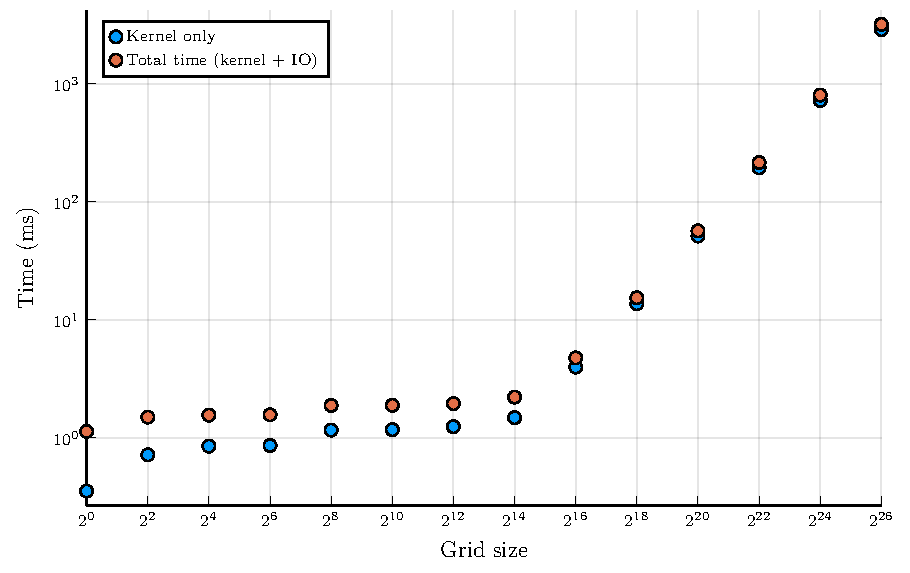
\includegraphics[width=1.0\textwidth]{e_time_kernel}
    \caption{Execution time of CUDA version with separate kernel time
    }%
    \label{fig:time_overhead}
\end{figure}

\Cref{fig:time_overhead} shows the execution time of the CUDA version with a
separate measure for the time spent in the kernel (the actual calculation). Total
time is the time spent in the kernel plus the additional time for input/output
operations and CUDA synchronization directives. For grid sizes of 1 and 2, most of the
time is spent outside the kernel. We can observe that the time is roughly the same
from grid sizes $1$ to $2^14 (16384)$ but after that there is a notable increase.
This is due to the fact the GPU used has 10240 CUDA cores so
we are using all cores and reaching the parallelization limit of the device.

If we now add the execution time of the \emph{C} sequential implementation of the
program we obtain~\cref{fig:time_cuda}. The CUDA version outperforms the sequential
version for grid resolutions as low as $4\times4$. This is due to the nature of the
computation which has very little overhead on copying operations between the GPU and
CPU, allowing for really notable performance gains. The quadratic fit on the sequential time
shows how it increases quadratically with the grid resolution.

\begin{figure}[H]
    \centering
    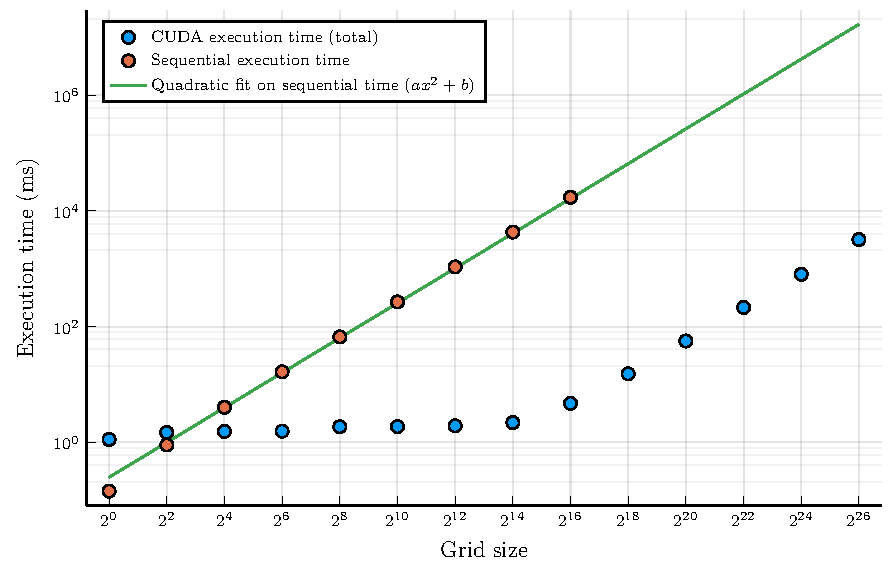
\includegraphics[width=1.0\textwidth]{e_time_all}
    \caption{Execution time of CUDA version vs. Sequential}%
    \label{fig:time_cuda}
\end{figure}

\begin{figure}[H]
    \centering
    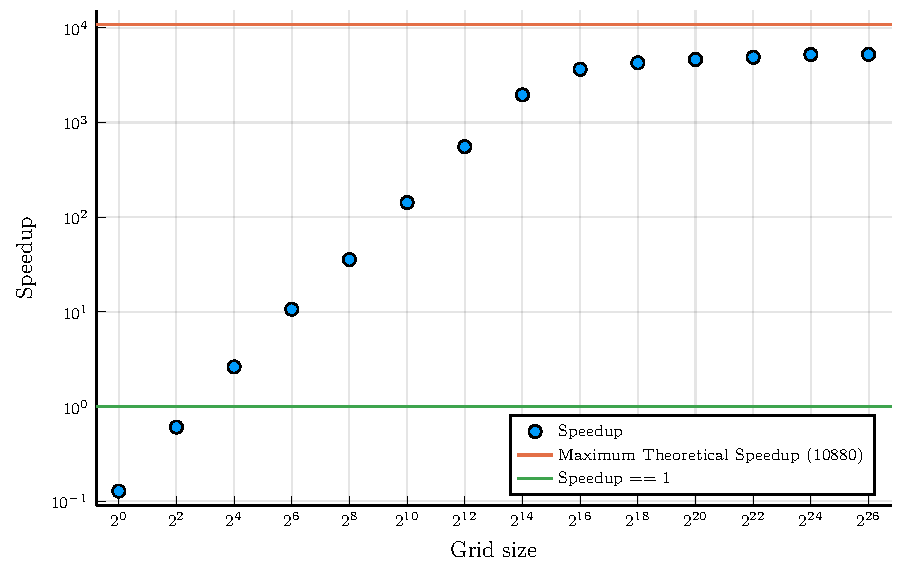
\includegraphics[width=1.0\textwidth]{speedup}
    \caption{Speedup of CUDA version vs. Sequential}%
    \label{fig:speedup}
\end{figure}

% {\bf define speedup ???}

By computing the ratio between the execution time of the sequential version and the CUDA
version, we obtain the \emph{Speedup}, which indicates how much faster the CUDA computation is
compared to the sequential version. As stated before the GPU used has 10240 cores so the
theoretical maximum speedup is 10240. Obviously such speedup is not feasible, both due to the
fact that a CPU core runs faster than a CUDA core and that there are additional operations
of communication between CPU and GPU that increase the execution time.
The dependence of the speedup on the number of trajectories is shown in \cref{fig:speedup}.

The overhead for starting CUDA processes make the GPU code slower for
calculation of small number of trajectories. For $\approx 2^4 = 16$ trajectories
the parallel and the serial codes require a similar execution time. The parallel
code runs faster (speedup larger than one) for larger number of trajectories.
The theoretical maximum for speedup is limited by the number of cores in GPU
(10240 in the present case) while here we observe $5239$ at maximum. There is
still an order of magnitude from the maximum achievable speedup which gives room
for improvement. Specially if we use additional GPUs. For reference, the
computation of $2^{26} \approx 6\times 10^7$ trajectories took 3.202s on the GPU
while the sequential version of the program would take approximately 4 hours and
40 minutes.  This massive computation of $2^{26}$ trajectories requires around 7
Gb of GPU memory if using and polynomial interpolation (although there is only
550Mb of data to needed for the final result). Given that the GPU has 12 Gb of
memory, higher resolutions cannot be performed with this kernel.

% {\bf ??? check how i changed the text}
